\documentclass[12pt]{article}
\usepackage[utf8]{inputenc}
\usepackage{amsmath}
\usepackage{graphicx}
\usepackage{hyperref}
\usepackage{listings}

\setlength{\parindent}{0pt}
\title{ERTS: Assignment 1}
\author{
Simon Møller, student number: 202204535 \\ 
Mark Myrtoft Bøgelund, student number: 202206634
}
\date{Date: \today}
\lstset{
    language=C++,
    basicstyle=\ttfamily\small,
    frame=single,
    breaklines=true
}

\begin{document}
\maketitle

\section*{Introduction}
This journal documents the SystemC models developed for Assignment 1. The exercises cover event-driven processes, FIFO communication, and cycle-accurate Avalon Streaming communication.

\newpage
\section*{Exercise 3.1: ModuleSingle}
\textbf{Task.} Create a module with a thread and a method. The thread should notify the method every 2 ms, and the method should increment and print an \texttt{sc\_uint<4>} counter during a 200 ms simulation.

\textbf{Solution.} The implemented clock-sensitive thread increments the four-bit counter and prints its value at every positive clock edge. Its 4-bit range is 0--15, so incrementing 15 wraps the counter to 0.

\begin{lstlisting}[caption={Clock-sensitive counter thread in ModuleSingle.}, label={lst:modulesingle-counter}]
void notify()
{
    while (true)
    {
        counter++;
        std::cout << "Time:"
                  << sc_time_stamp()
                  << "| Counter: "
                  << counter
                  << std::endl;
        wait();
    }
}

SC_THREAD(notify);
sensitive << clk.pos();
\end{lstlisting}

As seen in Listing~\ref{lst:modulesingle-counter}, the process increments and prints the counter before waiting for the next clock edge.

\begin{figure}[htbp]
    \centering
    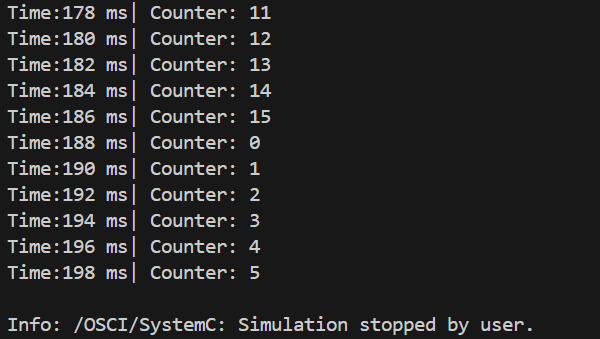
\includegraphics[width=0.9\textwidth]{images/sim-res-1.png}
    \caption{ModuleSingle simulation output. The counter wraps from 15 to 0 at 188 ms.}
    \label{fig:modulesingle-result}
\end{figure}

As seen in Figure~\ref{fig:modulesingle-result}, the counter reaches 15 and wraps to 0 at 188 ms, then continues counting.

\clearpage
\section*{Exercise 3.2: ModuleDouble}
\textbf{Task.} Model two threads that notify events A and B every 3 ms and 2 ms, respectively. A method must acknowledge the event and alternate dynamically between waiting for A and B.

\textbf{Solution.} Each branch of the method prints the received event, notifies its acknowledgement event, and uses \texttt{next\_trigger()} to make the other event the next trigger.

\begin{lstlisting}[caption={Dynamic event selection and acknowledgement in ModuleDouble.}, label={lst:moduledouble-events}]
if (waitForA)
{
    std::cout << "Time: " << sc_time_stamp() << " | Event: A" << std::endl;
    eventAack.notify();
    waitForA = false;
    next_trigger(eventB);
}
else
{
    std::cout << "Time: " << sc_time_stamp() << " | Event: B" << std::endl;
    eventBack.notify();
    waitForA = true;
    next_trigger(eventA);
}
\end{lstlisting}

As seen in Listing~\ref{lst:moduledouble-events}, receiving A selects B as the next trigger, while receiving B selects A. Each event is acknowledged before the switch.

\begin{figure}[htbp]
    \centering
    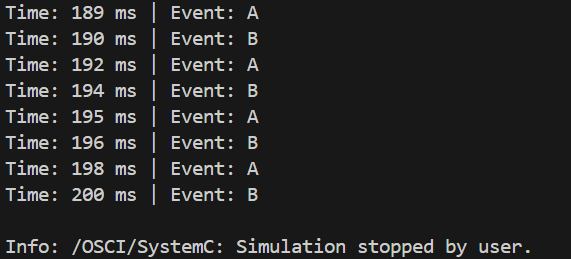
\includegraphics[width=0.9\textwidth]{images/sim-res-2.png}
    \caption{ModuleDouble simulation output. Events A and B alternate until the 200 ms simulation limit.}
    \label{fig:moduledouble-result}
\end{figure}

As seen in Figure~\ref{fig:moduledouble-result}, the method alternates between A and B notifications, reaching the 200 ms simulation limit.

\clearpage
\section*{Exercise 3.3.1: FIFO communication}
\textbf{Task.} Connect a producer and a consumer using an \texttt{sc\_fifo}. The producer must transmit TCP-header packets at random intervals, and the consumer must report each received packet.

\textbf{Solution.} The producer allocates and initializes a \texttt{TCPHeader}, writes it to the FIFO, and waits for a random delay. The blocking \texttt{read()} in the consumer synchronizes receipt with packet availability; the consumer then prints the payload and releases the allocated packet.

\begin{lstlisting}[caption={Creation and FIFO transmission of a TCP-header packet.}, label={lst:fifo-producer}]
TCPHeader *val = new TCPHeader();
val->SourcePort = 1234;
val->DestinationPort = 5678;
val->SequenceNumber = 1;

std::string data = "Hello, World!";
std::copy(data.begin(), data.end(), val->Data);
fifo_out.write(val);

int random_delay = rand() % 10 + 2;
wait(random_delay, SC_NS);
\end{lstlisting}

As seen in Listing~\ref{lst:fifo-producer}, the producer initializes a TCP header, writes it to the FIFO, and delays before producing the next packet.

\begin{lstlisting}[caption={Blocking receipt and deletion of a TCP-header packet.}, label={lst:fifo-consumer}]
TCPHeader *val = fifo_in.read();
std::cout << "Read " << val->Data << " at " << sc_time_stamp() << std::endl;
delete val;
\end{lstlisting}

As seen in Listing~\ref{lst:fifo-consumer}, the consumer waits for a packet, prints its payload and simulation time, then releases its memory.

\begin{figure}[htbp]
    \centering
    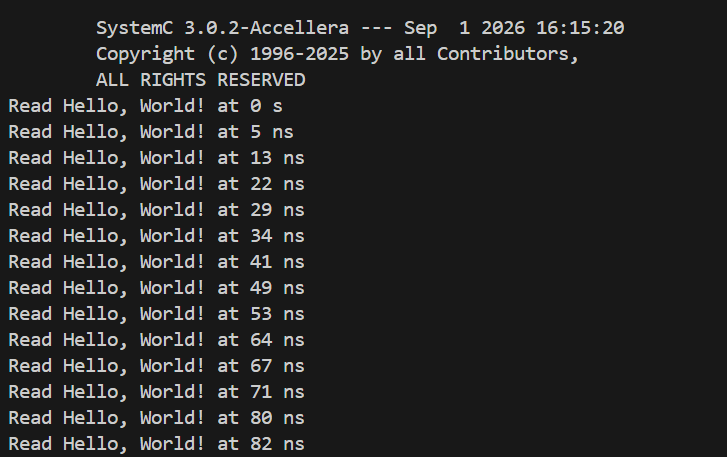
\includegraphics[width=0.9\textwidth]{images/sim-res-3.1.png}
    \caption{Single-consumer FIFO simulation output. The consumer receives packets after varying simulated delays.}
    \label{fig:fifo-single-result}
\end{figure}

As seen in Figure~\ref{fig:fifo-single-result}, the consumer receives each \texttt{Hello, World!} packet at non-uniform simulation times, reflecting the random producer delay.

\clearpage
\section*{Exercise 3.3.2: Two consumers}
\textbf{Task.} Extend the model with two FIFO channels and consumers. The producer must use a multiport and send a packet to each connected output.

\textbf{Solution.} The two-element FIFO output port is iterated, and a separately allocated TCP packet is written to each connected channel. The payload identifies the receiving consumer.

\begin{lstlisting}[caption={Multiport producer sends a packet to each connected FIFO channel.}, label={lst:fifo-two-consumers}]
sc_port<sc_fifo_out_if<TCPHeader *>, 2> fifo_out;

for (size_t i = 0; i < fifo_out.size(); ++i)
{
    TCPHeader *val = new TCPHeader();
    val->SourcePort = 1234;
    val->DestinationPort = 5678;
    val->SequenceNumber = 1;
    val->Acknowledge = 0;
    val->StatusBits = 0;
    val->WindowSize = 0;
    val->Checksum = 0;
    val->UrgentPointer = 0;

    std::string data = "Hello, consumer " + std::to_string(i + 1);
    std::copy(data.begin(), data.end(), val->Data);
    fifo_out[i]->write(val);
}
\end{lstlisting}

As seen in Listing~\ref{lst:fifo-two-consumers}, the producer iterates over its two FIFO outputs and creates a distinct packet for each consumer.

\begin{figure}[htbp]
    \centering
    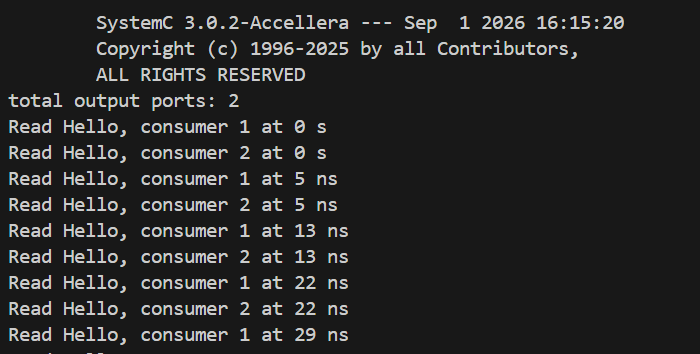
\includegraphics[width=0.9\textwidth]{images/sim-res-3.2.png}
    \caption{Two-consumer FIFO simulation output. Both consumers receive their individual packet at each transmission time.}
    \label{fig:fifo-two-consumers-result}
\end{figure}

As seen in Figure~\ref{fig:fifo-two-consumers-result}, consumer 1 and consumer 2 receive their corresponding packets at the same simulation times.

\clearpage
\section*{Exercise 3.4: Avalon Streaming master and slave}
\textbf{Task.} Create a cycle-accurate master/slave model using Avalon Streaming signals. The model must include \texttt{valid}, \texttt{ready}, data, channel, and error signals, and create a VCD waveform trace.

\textbf{Solution.} The master drives the data, channel, error, and \texttt{valid} signals, then waits until the slave asserts \texttt{ready}. The slave module records all interface signals in the \texttt{WaveForm} VCD trace for GTKWave inspection.

\begin{lstlisting}[caption={Master drives Avalon-ST data and waits for the ready handshake.}, label={lst:avalon-master}]
data.write(i);
channel.write(i % MAX_CHANNEL);
error.write(0);
valid.write(true);

wait();

while (!ready.read())
{
    wait();
}

valid.write(false);
\end{lstlisting}

As seen in Listing~\ref{lst:avalon-master}, the master keeps \texttt{valid} asserted until \texttt{ready} is observed, completing the Avalon-ST handshake.

\begin{lstlisting}[caption={VCD trace configuration for the Avalon-ST interface signals.}, label={lst:avalon-trace}]
tf = sc_create_vcd_trace_file("WaveForm");
tf->set_time_unit(1, SC_NS);
sc_trace(tf, clk, "clock");
sc_trace(tf, valid, "valid");
sc_trace(tf, data, "data");
sc_trace(tf, channel, "channel");
sc_trace(tf, error, "error");
sc_trace(tf, ready, "ready");
\end{lstlisting}

As seen in Listing~\ref{lst:avalon-trace}, the VCD trace contains the clock and every signal needed to inspect the transfer handshake in GTKWave.

\begin{figure}[htbp]
    \centering
    \fbox{\parbox[c][4cm][c]{0.85\textwidth}{\centering [SIMULATION RESULT]}}
    \caption{GTKWave view of the Avalon-ST clock, valid, ready, data, channel, and error signals.}
    \label{fig:avalon-result}
\end{figure}

As seen in Figure~\ref{fig:avalon-result}, the GTKWave screenshot will show the timing relationship between \texttt{valid}, \texttt{ready}, and the transmitted data signals.

\end{document}
